\chapter{Reconnaissance des chiffres manuscrits}

\section{La base de données MNIST}

\subsection{Présentation de MNIST}
La base de données MNIST (ou Mixed National Institute of Standards and Technology) est un regroupement de 70 000 chiffres manuscrits. 60 000 d'entre eux servent à l'apprentissage et les 10 000 autres permettent de tester le réseau de neurones après l'apprentissage. Ce sont des images normalisées en noir et blanc, de 28 pixels de côté chacun codé sur un octet. Nous nous appuierons sur cette base de données pour faire apprendre à notre réseau de neurones la reconnaissance de chiffres.

\begin{figure}[h]
\begin{center}
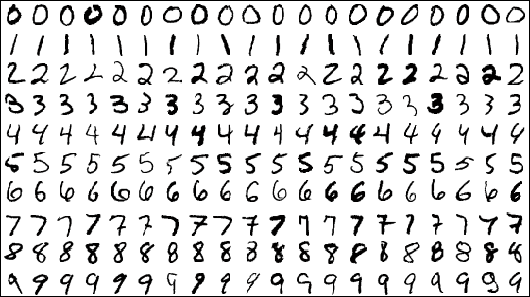
\includegraphics[width=0.6\textwidth]{images/mnistExamples.png}\caption{Exemples d'images tirées de la base de données MNIST. Chaque chiffre fait 28 pixels de côté}
\end{center}
\end{figure}

\subsection{Extraction de MNIST} 
Les données sont dans le format idx1 et idx3 tel que : \\ \\
\begin{tabular}{|c | c | c | c|}
\hline
\textbf{offset} & \textbf{type} & \textbf{valeur} & \textbf{description} \\
\hline
0000 & 32 bit integer & 0x00000803(2051) & magic number\\
0004 & 32 bit integer & 60000 & number of items\\
0008 & 32 bit integer & 28 & number of rows \\
0012 & 32 bit integer & 28 & number of columns \\
0016 & unsigned byte & ?? & pixel\\
0017 & unsigned byte & ?? & pixel\\
... & ... & ... & ... \\
xxxx  &  unsigned byte & ?? & pixel\\
\hline
\end{tabular} \\ \\
On peut distinguer :
\begin{itemize}
  \item Le \textit{magic number} qui permet d'identifier le format de la base de données
  \item Les \textit{number of items, number of rows, number of colums} donne des informations sur les données, ce qui nous permettra d'extraire les images
  \item Les \textit{pixels} qui sont les octets en niveau de gris des images
\end{itemize} 
L'extraction se fait donc en lisant successivement les octets et en les stockant dans des \textit{vector<Eigen:Matrix>} grâce aux données récupérées. En faisant de même avec les labels dont le format est très sensiblement le même, on obtient une liste de vecteur colonne d'\textit{Eigen::Matrix} de taille 784 (28*28) ainsi que leur label sur un autre \textit{Eigen::Matrix}. On fait de même avec les échantillons de test et on est fin prêt pour l'apprentissage.

\section{Apprentissage de la base de données}
\subsection{Paramétrage du réseau de neurones}
Bien que le format de l'entrée soit le même que pour le XOR (vecteur colonne si ce n'est la taille qui change), un réseau à 3 ou 4 neurones ne suffit pas. Il a fallu adapter de façon empirique les différents paramètres. On peut jouer sur :
\begin{itemize}
  \item Le nombre de neurones par couche
  \item Le nombre de couches
  \item Le pas d'apprentissage
  \item Les fonctions d'activations par couches
  \item Le nombre d'apprentissages
\end{itemize}
\subsubsection{Le nombre de couches et de neurones}
Dans le cas d'un perceptron, nous avons réussi à obtenir un réseau classificateur de chiffre à 90\% de succès avec uniquement une couche composée de 10 neurones. Néanmoins, afin d'obtenir un score de réussite supérieur, il a été nécessaire de d'augmenter la nombre de couche à 3, selon une configuration $784\times300\times100\times10$ où 784 représente le nombre d'entrée.
\subsubsection{Le pas d'apprentissage}
Le pas d'apprentissage par défaut utilisé avec succès sur le XOR était de $\eta=0,01$. Or, pour MNIST, un pas de $\eta=0,01$ ne permet pas au réseau de sortir d'un minimum local. Un pas fonctionnel était de $\eta=0,2$
\subsubsection{Les fonctions d'activations par couches}
Nous avons, comme dans le cas du XOR (cf. \ref{subsec:XOR_Résolution}), continué à utiliser un fonction d'activations sigmoïde pour toutes les couches : $\frac{1}{1+exp(-\lambda x)}$, avec cette fois-ci $\lambda=0,1$
\subsubsection{Le nombre d'apprentissages}
Le nombre d'apprentissage nécessaire pour obtenir un taux d'erreur inférieur à 10\% est relativement important, notamment par rapport au nombre d'apprentissages nécessaire au GAN, aux alentours de 250 000 apprentissages. Néanmoins, passé ce nombre d'apprentissage, la courbe d'apprentissage varie peu. Il est nécessaire d'effectuer environ un million d'apprentissages pour avoir un taux d'erreur de 5\%. Ces résultats ont été effectués avec des descentes de gradients classiques sur le réseau à 3 couches cité plus haut.
\subsection{Résultat}
On peut voir le résultat sur la figure \ref{fig:res_MNIST}
\begin{figure}[h]
\begin{center}
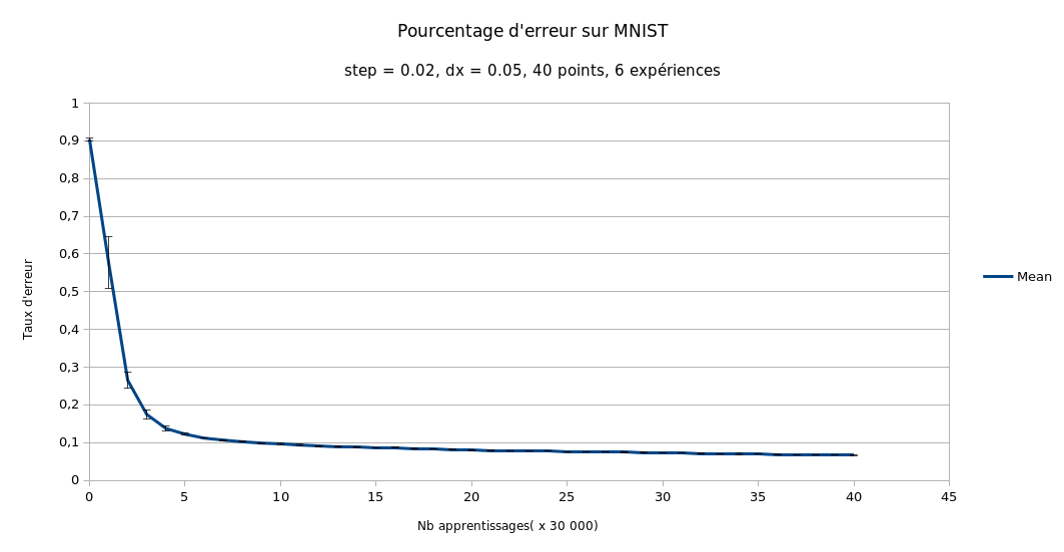
\includegraphics[width=1\textwidth]{images/courbe_MNIST.png}
\caption{Courbe du taux d'erreur de MNIST}
\label{fig:res_MNIST}
\end{center}
\end{figure}
